\documentclass[oneside,11pt,openright]{report}

\usepackage[latin1]{inputenc}
\usepackage[american]{babel}
\usepackage{a4}
\usepackage{latexsym}
\usepackage{amssymb}
\usepackage{amsmath}
\usepackage{epsfig}
\usepackage[T1]{fontenc}
\usepackage{lmodern}
\usepackage[labeled]{multibib}
\usepackage{color}
\usepackage{datetime}
\usepackage{epstopdf} 
\usepackage{graphicx}

\usepackage{pgf,tikz}
\usepackage{comment}
\usetikzlibrary{arrows,automata}
\usetikzlibrary{backgrounds,fit}
\usetikzlibrary{shapes,patterns}
\usetikzlibrary{calc,chains,positioning}

\renewcommand*\ttdefault{txtt}
\newcommand{\BigO}[1]{\ensuremath{\operatorname{O}\left(#1\right)}}
\newcommand{\BigT}[1]{\ensuremath{\Theta\left(#1\right)}}
\newcommand{\specialcell}[2][c]{%
  \begin{tabular}[#1]{@{}c@{}}#2\end{tabular}}
% see http://imf.au.dk/system/latex/bog/

\newcommand{\adjustimg}{% Horizontal adjustment of image
  \ifodd\value{page}\hspace*{\dimexpr\evensidemargin-\oddsidemargin}\else\hspace*{-\dimexpr\evensidemargin-\oddsidemargin}\fi%
}
\newcommand{\centerimg}[2][width=\textwidth]{% Center an image
  \makebox[\textwidth]{\adjustimg\includegraphics[#1]{#2}}%
}
\newcommand{\MakeHeap}{\textsc{MakeHeap}}
\newcommand{\FindMin}{\textsc{FindMin}}
\newcommand{\Insert}{\textsc{Insert}}
\newcommand{\DeleteMin}{\textsc{DeleteMin}}
\newcommand{\DecreaseKey}{\textsc{DecreaseKey}}
\newcommand{\Delete}{\textsc{Delete}}
\newcommand{\Meld}{\textsc{Meld}}
\newcommand{\Dijkstra}{\textsc{Dijkstra}}
\newcommand{\NULL}{\textbf{null}}

\begin{document}

%%%%%%%%%%%%%%%%%%%%%%%%%%%%%%%%%%%%%%%%%%%%%%%%%%%%%%%%%%%%%%%%%%%%%%%

\pagestyle{empty} 
\pagenumbering{roman} 
\vspace*{\fill}\noindent{\rule{\linewidth}{1mm}\\[4ex]
  {\Huge\sf Binary Heaps, Fibonacci Heaps and\\[2ex]Dijkstras shortest path}\\[4ex]
  {\huge\sf Kristoffer Just Andersen, 20051234\\[2ex]
    \huge\sf Troels Leth Jensen, 20051234 \\[2ex]
    \huge\sf Morten Krogh-Jespersen, 20022362}\\[2ex]
  \noindent\rule{\linewidth}{1mm}\\[4ex]
  \noindent{\Large\sf Project 1, Advanced Data Structures 2013, Computer Science\\[1ex] 
    \monthname\ \the\year  \\[1ex] Advisor: Gerth St�lting Brodal\\[15ex]}\\[\fill]}
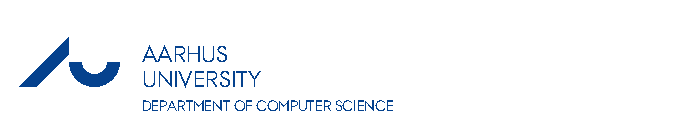
\epsfig{file=logo.eps}\clearpage

%%%%%%%%%%%%%%%%%%%%%%%%%%%%%%%%%%%%%%%%%%%%%%%%%%%%%%%%%%%%%%%%%%%%%%%

\tableofcontents
\pagenumbering{arabic}
\setcounter{secnumdepth}{2}

%%%%%%%%%%%%%%%%%%%%%%%%%%%%%%%%%%%%%%%%%%%%%%%%%%%%%%%%%%%%%%%%%%%%%%%

\chapter{Introduction}

This report details our investigation into the performance
characteristics of the heap data structure. The heap can be used as a
minimum priority queue, a use applicable in a wide variety of problem
domains: process scheduling, sorting and graph algorithms all have a
place for heaps.

This paper will explore two general approaches, the binary and
Fibonacci heaps, and demonstrate two ways of implementing each, for a
total of four different data structures. We argue for their worst case
time behaviour.

We then put them to the emprical test, stressing them under load from
Dijsktra's Single Source Shortest Path algorithm, which we use to
demonstrate the performance characteristics of the data
structures. Dijsktra's can be implemented in two different ways, and
we investigate the consequence of one method over the other.

%%%%%%%%%%%%%%%%%%%%%%%%%%%%%%%%%%%%%%%%%%%%%%%%%%%%%%%%%%%%%%%%%%%%%%

\chapter{Binary heaps}

This chapter explores binary heaps as presented in
\cite{Forsythe:1964}. A binary heap gets its name from the balanced,
binary search tree over its elements that it maintains. We shall see
two ways to achieve this, one maintaining an explicit search tree, the
other relying on the isomorphism between arrays and balanced trees.

The key to using a binary tree for the purpose of a priority que is
the ``heap invariant'': that the priority of each element in the tree
is smaller than its children. Maintaining this invariant is the focus
of each operation on binary heaps, and the notion of ``bubbling''
elements up and down through the tree, swapping children and parents,
appears again and again, as we shall see. We begin with an overview of
the running times of each of the two implementations we investigate.

\begin{center}
  \begin{tabular}{ l | c | c  }
    Operation & Array Implementation & Pointer Based \\ \hline
    \MakeHeap & $\BigT{1}$ & $\BigT{1}$ \\ 
    \FindMin & $\BigT{1}$ & $\BigT{1}$\\
    \Insert & $\BigO{n}$ & $\BigT{\log n}$ \\ 
    \DeleteMin & $\BigT{\log n}$ & $\BigT{\log n}$ \\
    \DecreaseKey & $\BigT{\log n}$ & $\BigT{\log n}$ \\
  \end{tabular}
\end{center}


\section{Binary Heaps with Arrays}

The original paper from 1964 utilizes the balanced binary tree implied
by the order of elements in an array. If we label the elements in the
array from 1, we see that they correspond uniquely to a position in
the following binary tree:

\begin{center}
  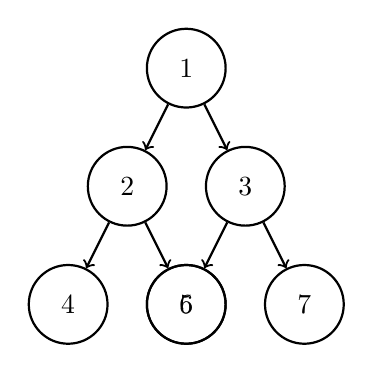
\begin{tikzpicture}[thick,->,auto,node distance=4cm]
    \tikzstyle{node}=[circle, minimum size=1cm, draw]
    
    \node[node]    	  (1) {$1$}
    child{node[node]      (2) {$2$}
      child{node[node]    (4) {$4$}}
      child{node[node]    (5) {$5$}}}
    child{node[node]      (3) {$3$}
      child{node[node]    (6) {$6$}}
      child{node[node]    (7) {$7$}}};
    
  \end{tikzpicture}
\end{center}


The parent-child relationships in the tree can be seen in the array by
observing that the numbers of node $i$s children are $2i$ and $2i +
1$. Similarly, the parent of node $i$ is node
$\left\lfloor\frac{i}{2}\right\rfloor$. Therefore, if the
implementation language supports arrays, there is no need to maintain
an explicit representation of a binary tree, likely saving space and
time.

It is of course entirely possible to take the alternate approach,
which we investigate in the next section.

\section{Implementation Decisions}

The algorithms used in our C implementation are faithful to the paper,
save for slight modernizations such as removal of \texttt{goto}
statements in favor of familiar looping control flow. This does not
alter the asymptotic running times or space consumption of the
algorithm.

We choose to inline the \textsc{Swopheap} operation as used by
\cite{Forsythe:1964}, as we believe it makes the intent
clearer. \textsc{Swop} has the effect of ``bubbling'' an element down
through the heap until the heap invariant is reestablished. This is
used for \DeleteMin, where the root of the tree is removed and replaced
by the last leaf of the tree, which is then bubbled downwards.

For the \DecreaseKey\ operation, we refer to Cormen \emph{et al.} \cite{ITA09}, which
demonstates an implementation of maximum priority queues supporting an
\textsc{IncreaseKey} operation. It is easy to transfer the algorithm
to our implementation. The basic algorithm decreases they key of an
element, and then proceeds to bubble the element up through the heap
until the heap invariant is reestablished, similar to how the original
implementation achieves insertion.

\section{Time-complexity for Binary Heaps with Arrays}

We here present arguments for the worst-case running times of the
following operations: \MakeHeap, \FindMin, \Insert, \DeleteMin and
\DecreaseKey - the operations we need to implement Dijkstra's
Algorithm in later sections.

\paragraph{\MakeHeap} Runs in constant time: \BigO{1}. All we do is a
single allocation of contiguous memory to store the elements of the
heap.

\paragraph{\FindMin} Runs in constant time: \BigO{1}. We do a single array
indexing, as, according to our heap invariant, the element of lowest
key is always in root position - the first element in our underlying
array.

\paragraph{\Insert} Runs linearly in the number of elements in
the heap: \BigO{n}. We insert the incomming node into the last position
of the tree, which we know by maintaining the current element
count. We then bubble the element upwards, performing a comparison and
a swap per level it moves. Thus we achieve a logarithmic running time
as the depth of a balanced binary tree is proportional to $\log
n$. However, due to the workings of C, we cannot dynamically alter the
size of the underlying array, and so, worst-case, we have to
reallocate the entire underlying array. We use the same approach as
the standard Java ArrayList of doubling the underlying array each time
the limit is reached. This requires copying the entire array, byte by
byte, into a new array, an operation linear in the number of elements,
which dominates the logarithmic cost of maintaining the heap
invariant. While this is a worst-case analysis, it is worth noting
that the amortized cost is \BigO{1}, where we pay for the cost of
reallocation by paying more per insertion.

\paragraph{\DeleteMin} Runs logarithmically in the number of elements
inserted: $O(\log n)$. We Remove the minimal element according to
\FindMin and replace it as root with the last element in the tree
(always found at position \textsc{Size} in the array). We then bubble
the element down through the tree, at most two comparisons and a swap
per level in the tree. The depth of a balanced binary tree is $O(\log
n)$. So we do a constant amount of work per level the node moves,
resulting in the logarithmic running time.

\paragraph{\DecreaseKey} Runs logarithmically in the number of
elements inserted: \BigO{\log n}. We decrease the key of the specified
element, and proceed to bubble it upwards until the invariant is
reestablished, using a single comparison and a swap per level
moved. The argument is similar to the one used for insertion and
deletion.

\section{Binary Heaps with Pointers}

While the original implementation used an underlying array, it is not
strictly necessary to achieve the benefit of a binary heap. We can
model the balanced binary tree explicitly using pointers. 

The algorithms follow the same procedures operationally as described
above, but with slight variations since we loose the direct access to
arbitrary positions in the tree facilitated by an underlying
array. Instead we must ``count'' our way into the tree.

The ``trick'' to achieve the same, if not better, running times as the
original implementation, is observing that position of a node $i$ in
the tree is given uniquely by the binary representation of $i -
1$. Read from most significant bit, the ones and zeroes gives
``directions'' from the root to the particular node. We defer to the
implementation for the goary details.

\section{Time-complexity for Binary Heaps with Pointers}

We here detail the worst case running times for the key operations of
a minimum priority que: \MakeHeap, \FindMin, \Insert, \DeleteMin and
\DecreaseKey.

\paragraph{\MakeHeap} Runs in constant time: \BigO{1}. Allocation of
the necessary varibales for keeping count of the elements inserted and
a pointer to the root node, once inserted.

\paragraph{\FindMin} Runs in constant time: \BigO{1}. By maintaining a
pointer to the root node, we have constant time access to it.

\paragraph{\Insert} Runs logarithmically in the number of elements:
\BigO{\log n}. Ny maintaining the number of elements inserted, we
can calculate directions to the position of the next element. This
involves reading bits and following pointers. We follow one pointer
per bit of ``direction''. The binary representation of $n$ uses $\log
n$ bits, so we follow \BigO{\log n} pointers. Upon insertion, we then
bubble the element up to reestablish the heap invariant, swapping
appropriate pointers as we go. We do this a number of times
proportional to the depth of the tree. Thus we run in time
$\BigO{2\log n} = \BigO{\log n}$.

\paragraph{\DeleteMin} Runs logarithmically in the number of elements:
\BigO{\log n}. Similarly to \Insert, we can find the last element in the
heap by tracing a path down from the root. This is logarithmic in the
number of elements for the same reasons. Then, we swap the root and
the last element, and bubble the last element down until the heap
invariant is restored. This is also logarithmic in the number of
elements.

\paragraph{\DecreaseKey} Runs logarithmically in the number of
elements: \BigO{\log n}. We decrease the key of the specified element,
and bubble upwards until we reestablish heap order. This is
proportional to the depth of the tree and thus logarithmic in the
number of elements.

\section{Correctness of Binary Heaps}

We opted for a visual inspection rather than unit testing. We
implement a \texttt{to\_dot} procedure that serializes a heap in the
form of a GraphViz dot file, from which we can render an image of the
associated binary tree. The procedure traverses the actual tree
structure recursively in the case of the pointer based implementation,
while calculating the implicit binary tree in the case of the array
based implementation.

This gives us quick and easy visual feedback, which is invaluable
particularly in the case of the pointer based implementation. Between
two nodes, we have a total of 4 children pointers and 6 parent
pointers that needs to be updated, which is a lot for any programmer
to manage at a single time. Visualizing the pointers gave us
immeadiate feedback when on a by-need basis testing proved
discrepancies in behaviour.

\chapter{Fibonacci heaps}

In this chapter we focus on Fibonacci heaps, which is a data structure that has a forest of rooted trees as opposed to a binary heap that only has one tree \cite{FT87}. The data structure was invented by Michael L. Fredman and Robert Endre Tarjan and was published in the Journal of ACM in 1987. It has it name because the size of any subtree in a Fibonacci heap will be lower bounded by $F_{k+2}$ where $k$ is the degree of the root in that subtree and $F_k$ is the kth Fibonacci number. Below is the time-complexities of each of the heap operations listed:

\begin{center}
  \begin{tabular}{ l | c | c | c }
    Operation & Binary heap & \specialcell{Fibonacci heap v1\\(amortized)} & \specialcell{Fibonacci heap v2\\(amortized)} \\ \hline
    \MakeHeap & $\BigT{1}$ & $\BigT{1}$ & $\BigT{1}$ \\ 
    \FindMin & $\BigT{1}$ & $\BigT{1}$ & $\BigO{l(\log (\frac{n}{l}) + 1)}$\\ 
    \Insert & $\BigT{\log n}$ & $\BigT{1}$ & $\BigT{1}$ \\ 
    \DeleteMin & $\BigT{\log n}$ & $\BigO{\log n}$ & $\BigT{1}$  \\ 
    \DecreaseKey & $\BigT{\log n}$ & $\BigO{1}$ & $\BigO{1}$ \\ 
    \Delete & $\BigT{\log n}$ & $\BigO{\log n}$ & $\BigT{1}$ \\ 
    \Meld & $\BigT{n}$ & $\BigT{1}$ & $\BigT{1}$ \\
  \end{tabular}
\end{center}

\section{Properties of the Fibonacci heap}

The Fibonacci heap is a heap that has better amortized bounds than binary heaps, and one of the reasons to this is that some of the operations are lazy. We will later see that this has a big impact on worst-case time complexities for the operations that do the heavy lifting.

The heap maintains a collection of root nodes in a doubly linked circular list that supports inserting, joining and single deletions in constant time. Each node has a left and a right sibling pointer that facilitates the circular doubly linked list, a pointer to the parent and a pointer to an arbitrary child. If there is no parent or child the pointers point to \NULL. A node is marked if it has had a child removed. If a child is removed from a parent that is already marked the parent will be moved to the root and the parents parent will be marked or moved. A mark on a node is removed when it is added as a child to another node.

Items added to the heap are added as single-item trees rooted with a node for the corresponding item. It is only when performing a linking step that trees grow. Therefore, the degree of nodes can only change when linking, removing or decreasing the key of an item, since decreasing the key of an item cuts the node from its parent and move the node up to be joined with the roots. 

The upper bound $D(n)$ on the degree of any node of an n-node Fibonacci is $\BigO{\log n}$~\cite[p.~523]{ITA09}~\cite[p.~604]{FT87}. This can be shown by first observing that the degree of any node $y$ in the Fibonacci heap is bounded by when it was inserted into the list of its parent $x$ childs, where $degree(x) = k$. When $y_i$ was linked to $x$, where $i$ declares when $y$ was added to the children list of $x$, $x$ and $y_i$ must have had the same degree which results in $degree(y_i) \le k - 1$. $y$ could have lost at most one child before it would be cut from $x$ resulting in $degree(y_i) \ge i - 2$ where $i = 1,2,\cdots,k$.

By three different induction proofs and the lemma described above, it can be shown that if $k = degree(x)$ for any node in a Fibonacci heap then $size(x) \ge F_{k+2} \ge \phi^k$, where $\phi = (1+\sqrt{5}) / 2$ also known as the golden ratio. Hereafter, showing the bound of $D(n)$ is straight forward:
\begin{gather*}
  n \ge size(x) \ge \phi^k \\
  \Downarrow \\
  k \le \lfloor \log_\phi n \rfloor    
\end{gather*}

\section{The potential method}

We will analyse the amortized running times of the Fibonacci heaps by using the potential function \cite[p.~215]{FT87}. A potential function maps a state of a data structure to a real number representing the potential contained in that data structure \cite[p.~459]{ITA09}. The amortized cost of an operation $c_i$ that transforms a data structure in state $D_{i-1}$ to $D_{i}$ is:
\begin{align*}
  \hat{c} = c_i + \Phi(D_i) - \Phi(D_{i-1})
\end{align*}
The amortized cost is therefore the cost of the operation $c_i$ plus the change in the potential. If the operation releases potential, the relased potential gets subtracted from the cost of the operation. For the Fibonacci heaps we define the potential function as:

\begin{align*}
  \Phi(H) = trees(H) + 2marked(H)
\end{align*}

Where trees define the number of trees/roots in the forest and marked is the number of marked nodes. The reason to why marked nodes contains two units of potential is that one unit pays for the cut and the other pays for the node to become a root and thereby form a new tree.

\section{Fibonacci heap version 1}

The first Fibonacci heap variant we present is the original version proposed in FT87. A potential function is used to analyze the perfomance, thus the above stated time-complexities are amortized.

Our implementation pretty much follows from the article, with few minor exceptions. The article do not specify exactly how a node is found from an item in constant time, so we decided to place a pointer on the item. Also, melding is not totally destructable since we join the heap in of the two existing heaps and return an arbitrary one. 

The article mentions that $\Delete$ takes $\BigO{1}$ if the node to remove is not the min-node and without cascading deletes. The children of the node to delete must be moved up onto the root which can only be done in constant time if every children has a pointer to a parent pointer. In this way, we only have to change one pointer to update all parent pointers for the children of the beforementioned node. Since the running time of the \Delete~operation is amortized $\BigO{\log n}$ we chose a simpler version where we just update all parent pointers one by one. As stated above $size(node) \le \BigO{\log n}$ so this only takes $\BigT{\log n}$ time.

\MakeHeap~constructs a new empty Fibonacci heap, which means there are not roots and no marked nodes. Therefore, the potential of the empty heap is 0 and constructing the heap can be done in constant time. \FindMin~does not alter the potential and is only a pointer lookup which clearly is also a constant time operation. \Insert~inserts a new root which increments the potential by one. Combine that with the actual cost which is $\BigO{1}$ the \Insert~operation is $\BigO{1}$. \Meld~can be carried out in $\BigO{1}$ actual time and since the change is:
\begin{align*}
  \Delta & = \Phi(H) - (\Phi(H_1) + \Phi(H_2)) = 0
\end{align*}
the \Meld~operation has time $\BigO{1}$.

When analyzing the amortized cost of $\DeleteMin$, let us say that the minimum node to delete is actually the node with degree $D(n)$ which is the upper bound on the maximum degree for any node. Setting the parent pointer to \NULL and concatinating each node with the root list takes constant time for each of the $D(n)$ children. 
The linking phase work on at most $D(n) + tress(H) - 1$ trees, since we have removed the minimum node from the root list and at most will be adding $D(n)$. We also join trees of same degree, but when two trees are joined only one will remain in the root list, so this can happen at most the number of roots in the root list. Therefore, the actual working time is $\BigO{D(n) + trees(H)}$.

The potential before the $\DeleteMin$ operation executues is $trees(H) + 2marked(H)$. After, at most $D(n) + 1$ roots will exist because all others would be removed during the linking phase and there is no change to marked nodes. Therefore, we have that:
\begin{align*}
  \DeleteMin & = \BigO{D(n) + trees(H)} + \left(\left(D(n) + 1\right) + 2marked(H)\right) \\
  & - \left(trees(H) + 2marked(H)\right) \\
  & = \BigO{D(n)} + \BigO{trees(H)} - trees(H) \\
  & = \BigO{D(n)}
\end{align*}
Actually, a slight subtlety is happening above. We can turn up the units that we pay to cover the hidden constant in $\BigO{trees(H)}$, which allows us to cancel those two terms out, resulting in an amortized running time of $\BigO{D(n)} \le \BigO{\log n}$.

$\DecreaseKey$ takes constant time for moving the node for the item with the decreased key to the root, but then $c$ cascading deletes can occur. Therefore, the actual time is $\BigO{c}$. The change is potential is:
\begin{align*}
  \Delta & = \BigO{trees(H) + (c - 1) + 1} + 2(marked(H) - (c-1) + 1) \\
  &- (trees(H) + 2marked(H) \\
  & = \BigO{trees(H) + c} + 2(marked(H) - c + 2) - (trees(H) + 2marked(H)) \\
  & = 4 - c
\end{align*}
Therefore, the amortized running time of $\DecreaseKey$ is $\BigO{c} + 4 - c = \BigO{1}$

Last, we have to cover the running time of $\Delete$. First, we cut the node and move the children to the root, which is at most $D(n)$ operations. Next, a chain of cascading deletes can occur where the length is $c$, making the actual time $\BigO{D(n) + c}$. The change in potential is as follows:
\begin{align*}
  \Delta & = \BigO{trees(H) + D(n) + c} + 2(marked(H) - c + 2) \\
  &- (trees(H) + 2marked(H) \\
  & = D(n) + 4 - c \\
\end{align*}
But as we showed for $\DecreaseKey$, the released potential pays for the cascading deletes, so we only have to pay the $D(n)$ for the actual time and $D(n)$ for the change in potential, which is $\BigO{D(n)} \le \BigO{\log n}$.

\section{Worst case time-complexity for Fib heap v1}

There are three operations where changes to the potential occurs, and thus, the stated times are amortized for $\DeleteMin$, $\DecreaseKey$ and $\Delete$. Below we illustrate the worst-case for each of these operations by showing a configuration and how that configuration can be obtained from a sequence of operations :

\subsection{Worst case time-complexity for $\DeleteMin$}

As we showed in the previous section the actual time for performing $\DeleteMin$ is $\BigO{D(n) + trees(H)}$. When linking trees the change in potential pays for $trees(H)$, therefore, it is in the amount of trees the worst case configuration for $\DeleteMin$ can be found. It is easy to see that the worst case is when all the nodes in the heap is at the root in a linked list:

\begin{center}
  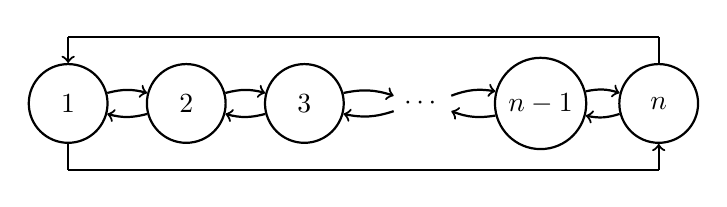
\begin{tikzpicture}[thick,->,auto,node distance=1.5cm]
    \tikzstyle{state}=[circle, minimum size=1cm, draw]
    
    \node[state]          (1) {1};
    \node[state]         (2) [right of=1] {2};
    \node[state]         (3) [right of=2] {3};
    \node          (dots) [right of=3] {$\cdots$};
    \node[state]         (nminusone) [right of=dots] {$n-1$};
    \node[state]         (n) [right of=nminusone] {$n$};
    \node          (dummy1) [below=0.2cm of 1] {};
    \node          (dummy2) [below=0.2cm of n] {};
    \node          (dummy3) [above=0.2cm of 1] {};
    \node          (dummy4) [above=0.2cm of n] {};
    
    \path (1)   edge [bend left=15] (2);
    \path (2) edge [bend left=15] (1);
    \path (2) edge [bend left=15] (3);
    \path (3) edge [bend left=15] (2);
    \path (3) edge [bend left=15] (dots);
    \path (dots) edge [bend left=15] (3);
    \path (dots) edge [bend left=15] (nminusone);
    \path (nminusone) edge [bend left=15] (dots);
    \path (nminusone) edge [bend left=15] (n);
    \path (n) edge [bend left=15] (nminusone);
    \path[-] (1) edge (dummy1.center);
    \path[-] (dummy1.center) edge (dummy2.center);
    \path (dummy2.center) edge (n);
    \path[-] (n) edge (dummy4.center);
    \path[-] (dummy4.center) edge (dummy3.center);
    \path (dummy3.center) edge (1);
  \end{tikzpicture}
\end{center}

This configuration can be achieved by just calling insert $n$ times. For simplicity, let us assume that $n$ is odd, and a call to $\DeleteMin$ happens. In the above example 1 will be removed and we are left with $n-1$ root nodes to link. This results in $n-1$ key comparisons, but all the trees of rank 1 will be joined too and this will continue until no trees of duplicate size is found.
\begin{align*}
  \text{\# of operations} = \BigO{n-1} + \BigO{\frac{n-1}{2}} + \BigO{\frac{n-1}{2^2}} + \cdots + \BigO{\frac{n-1}{2^{\log (n-1)-1}}}
\end{align*}
which is $\BigT{n}$.

\subsection{Worst case time-complexity for $\Delete$ and $\DecreaseKey$}

As we shoved in the previous section, the release in potential for cascading deletes pays for most of the work, therefore, we can find a worst-case configuration that will perform considerably worse in actual time.

If $\Delete$ is invoked with the min-node as argument then $\Delete$ calls $\DeleteMin$, therefore, the worst case for $\Delete$ is $\BigT{n}$, but we will show that without the min-node as argument, we still end up with $\BigT{n}$. The following observation holds true for $\DecreaseKey$ as well.

If we delete a child to an arbitrary node $x$ we mark $x$ if is not marked and if it is marked, we cut $x$ from its parent, move the subtree formed by $x$ to the root and try to mark the previous parent of $x$. This could result in cascading deletes. Therefore, the worst situation would be the following configuration:
\begin{center}
  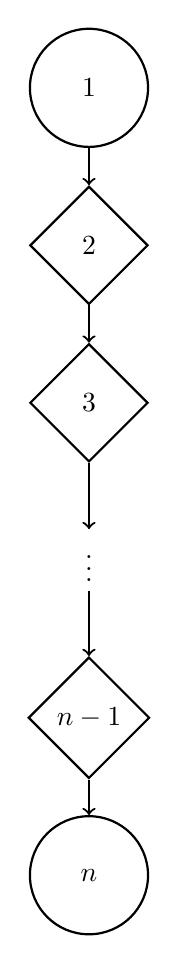
\begin{tikzpicture}[thick,->,auto,node distance=2cm]
    \tikzstyle{node}=[circle, minimum size=1.5cm, draw]
    \tikzstyle{marked}=[diamond, minimum size=1.5cm, draw]
    
    \node[node]    	  (1) {1};
    \node[marked]         (2) [below of=1] {2};
    \node[marked]         (3) [below of=2] {3};
    \node          (dots) [below of=3] {$\vdots$};
    \node[marked]         (nminusone) [below of=dots] {$n-1$};
    \node[node]         (n) [below of=nminusone] {$n$};
    
    \path (1) edge (2);
    \path (2) edge (3);
    \path (3) edge (dots);
    \path (dots) edge (nminusone);
    \path (nminusone) edge (n);

  \end{tikzpicture}
\end{center}

where a diamond is modelling a marked node. If either $\DecreaseKey$ or $\Delete$ is called with an item corresponding to node $n$ a cascading delete will begin and will not stop until it reaches $2$ in this example. The amount of operations is therefore the entire chain:
\begin{align*}
  \text{length of chain} = n - 1
\end{align*}
which is $\BigT{n}$.

Such a configuration can be obtained by calling $\Insert$ with two very high numbers $x$ and $y$ and one smaller and call $\DeleteMin$:

\begin{center}
  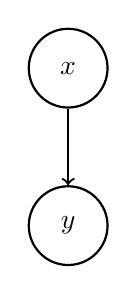
\begin{tikzpicture}[thick,->,auto,node distance=2cm]
    \tikzstyle{node}=[circle, minimum size=1cm, draw]
    \tikzstyle{marked}=[diamond, minimum size=1cm, draw]
    
    \node[node]    	  (1) {$x$};
    \node[node]           (2) [below of=1] {$y$};
    
    \path (1) edge (2);

  \end{tikzpicture}
\end{center}

If we insert three new items $x'$, $y'$ $z$ with keys slightly smaller where $z$ is the smallest key we will have the following forest:

\begin{center}
  \begin{tikzpicture}[thick,->,auto,node distance=2cm]
    \tikzstyle{node}=[circle, minimum size=1cm, draw]
    
    \node[node]    	  (x) {$x$};
    \node[node]           (y) [below of=x] {$y$};
    \node[node]    	  (x') [right of=x] {$x'$};
    \node[node]    	  (y') [right of=x'] {$y'$}; 
    \node[node]    	  (z) [right of=y'] {$z$};
    
    \path (1) edge (2);

  \end{tikzpicture}
\end{center}

If we call $\DeleteMin$, call $\Delete$ on $y'$ and call insert with three new items as above, we can get the following configuration:

\begin{center}
  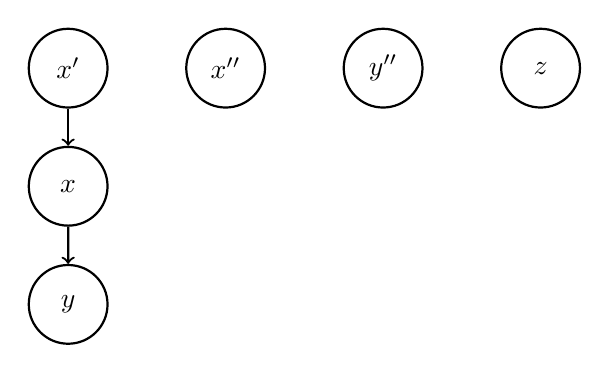
\begin{tikzpicture}[thick,->,auto,node distance=2cm]
    \tikzstyle{node}=[circle, minimum size=1cm, draw]
    
    \node[node]    	  (x') {$x'$}
    child{node[node]      (x) {$x$}
      child{node[node]    (y) {$y$}}};
    \node[node]    	  (x'') [right of=x'] {$x''$};
    \node[node]    	  (y'') [right of=x''] {$y''$}; 
    \node[node]    	  (z) [right of=y''] {$z$};
    
  \end{tikzpicture}
\end{center}
where $z$ again is the smallest key. $\DeleteMin$ gives:

\begin{center}
  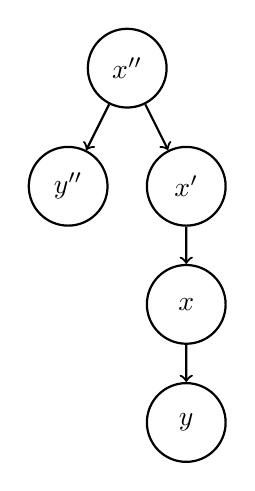
\begin{tikzpicture}[thick,->,auto,node distance=2cm]
    \tikzstyle{node}=[circle, minimum size=1cm, draw]
    
    \node[node]    	  (x'') {$x''$}
    child{node[node]      (y'') {$y''$}}
    child{node[node]      (x') {$x'$}
      child{node[node]    (x) {$x$}
        child{node[node]  (y) {$y$}}}};
    
  \end{tikzpicture}
\end{center}
where $\Delete$ with $y''$ as argument will result in a chain. By using this approach we can easily build up a single chain of height $n$.

\section{Fibonacci heap version 2}

In this second version of a Fibonacci heap we try to be more lazy, by doing as little work as possible for $\Delete$ and $\DeleteMin$. When a call to either one of the operations is called, we mark the node as vacant but then halt to do any additional work. This makes $\Delete$ and $\DeleteMin$ run in $\BigO{1}$.

We have to do some work at one point which happens in $\FindMin$. Now, $\FindMin$ works like $\DeleteMin$ in version 1, but also has to delete every vacant node it meets on the path. $\Meld$ also requires little work, such that when melding two heaps, if a root is marked as vacant it should be the new root of the resulting heap. There is no change in actual time for $\Meld$.

Below is an image from our test-framwork showing how a tree looks like with vacant nodes:

\mbox{} \par
\noindent\centerimg{delete_39.png}
After a call to $\FindMin$ thee heap looks like:

\mbox{} \par
\noindent\centerimg{find_min}

Let us analyze the time for the $\FindMin$ operation. Let $l$ mark the number of vacant nodes. If $l=0$ then $\FindMin$ points to the node representing the item with the minimum key, and the work is constant. If $l \ge 1$ then the amortized running time is the new roots created from destroying vacant nodes and moving the non-vacant child nodes to the root plus the linking of the trees which is at most $\BigO{\log n}$. We argued previously that a node $y$ have $degree(y_i) \ge i - 2$ for $i = 1,2,\cdots,k$ where $k$ is the degree of its parent. We use this to say that at least one of the vacant nodes will have a rank of $k-2$. We also know that the size of subtree rootet at a node with degree $k-2$ will be at least be of size $\phi^{k-2}$. If all children of the vacant nodes we destroy are nonvacant, they will increase the number of trees and thereby the potential by:
\begin{align*}
  \sum_{i=1}^l \phi^{k_j-2} \le n
\end{align*}
where $k_1, k_2,\cdots,k_i$ are nonvacant nodes. The sum is maximized for $k_i$. MAYBE SOME MORE??

\section{Worst case time-complexity for Fib heap v2}

The worst case example is extremely easy. Since $l$ and $n$ are disjoint, the can be filled with vacant nodes. The worst-case would then be calling $\FindMin$, just to find out that no such node exist. 

\section{Testing correctness of Fibonacci Heaps}

Implementing the Fibonacci heaps in C required a lot of work and since we are working with that many pointers, we decided very early in the proces that we needed some kind of test-framework to assist us. 

First, we implemented a consistency checker, that checks the following properties for each node $x$: That the nodes the sibling pointers of $x$ points to points to $x$ with the corresponding sibling pointer. That the parent pointer is correct if the node $x$ is a child of any node and that the key is larger than its parent. Still, this tests the implementation more than the properties of the Fibonacci heaps, so we needed one more tool.

We build a pretty printer that could convert any subtree (or heap) to a graphical representation, such that we could see how the heap looked like. We then made test-cases, that for each operation printed the output, and then we could manually check if $\DeleteMin$, $\Delete$ and $\DecreaseKey$ behaved as it should. We manually checked test-instances of size less than or equal to 100 operations.

Attached in the zipped-file companying the report are generated images we have used to check correctness.

Lastly, since we now have four datastructures, we could check the output for each and compare it with the others, to make sure, that all our heaps answer correctly (or all could answer wrong the same way, which is highly unlikely).

\chapter{Test-results}

needs content

\chapter{\Dijkstra's algorithm}

\Dijkstra's~algorithm is an graph search algorithm that can be used to
solve the single-source shortest path problem. Without a min-priority
queue, the algorithm runs in $\BigO{V^2} \ge \BigO{E}$ for a graph $G
=(V, E)$[3]. However, we have two heaps that can actually be used as
priority queues, so this will give us better asymptotic running times
depending on the connectivity of the graph.  Normally, $\Dijkstra$ is
implemented by using the $\DecreaseKey$ operation, but if we disregard
space, we can actually implement $\Dijkstra$ without $\DecreaseKey$
and just insert new nodes every time we find a shorter path. Below is
a summary of the time complexities follows:

\begin{center}
  \begin{tabular}{ l | c | c}
    Runtime of \Dijkstra & using \DecreaseKey & using \Insert \\ \hline
    Binary Heaps & $\BigO{(\mid V\mid+ \mid E \mid)\log \mid V\mid}$ &
    $\BigO{(\mid V\mid+ \mid E \mid)\log \mid V\mid}$\\
    Fibonacci v1 & $\BigO{(\mid V \mid+ \mid E \mid)\log \mid V
      \mid}$&$\BigO{(\mid V \mid+ \mid E \mid)\log \mid V
      \mid}$ \\
    Fibonacci v2 &$\BigO{(\mid V \mid+ \mid E \mid)\log \mid V
      \mid}$ &$\BigO{(\mid V \mid+ \mid E \mid)\log \mid V
      \mid}$
  \end{tabular}
\end{center}


We represent graphs with an adjacency matrix, which already consumes space $\BigO{n^2}$, so there will only be a constant increase if $\Dijkstra$ insert nodes as we go along.

\section{Connectivity and generating graphs}

\section{$\Dijkstra$ with \DecreaseKey}

\section{$\Dijkstra$ without \DecreaseKey}

\section{Expectations}

\chapter{Binary heap vs Fibonacci heap}

needs content

\chapter{Test-results}

needs content

\chapter{Conlusion}

needs contents


%%%%%%%%%%%%%%%%%%%%%%%%%%%%%%%%%%%%%%%%%%%%%%%%%%%%%%%%%%%%%%%%%%%%%%%

\addcontentsline{toc}{chapter}{Bibliography}
\bibliographystyle{plain} 
\bibliography{report}

\end{document}

